\documentclass[paper slide]{beamer}
\usetheme{Boadilla}
\usepackage{essay-def}
\usepackage{bm}
\usepackage{amsfonts}
\usepackage{amssymb}
\usepackage{amsmath}
\usepackage{amsthm}
\usepackage{comment}
\usepackage{subcaption}
\usepackage{geometry}
\usepackage{algorithmic}
\usepackage{algpseudocode}
\usepackage{algorithmicx}
\geometry{left=1cm,right=1cm}
    \title[]{Data-driven subgrid-scale modeling for wall turbulence}
\author[J. Zhao]{Jiaxi Zhao (NUS) \\ \small joint work with Sohei Arisaka (NUS) and Prof. Qianxiao Li (NUS)}
\date[\today]{The 19th OpenFOAM Workshop \\ \today}
\begin{document}
\par \setlength{\parindent}{2em}

\begin{frame}
\titlepage
\end{frame}

\begin{frame}{Motivation}
	
\end{frame}

\begin{frame}{SGS stress modeling}
	There are three main issues for stress modeling:
	\begin{itemize}
		\item The mapping from the input features. e.g. filtered velocity to the stress tensor is non-deterministic while
		most classical turbulence models and data-driven models are deterministic.
		\item 
	\end{itemize}
\end{frame}

\begin{frame}{Learning the SGS stress model}
	We test the following three approaches:
	\begin{itemize}
		\item 1. Directly predict the stress tensor from the input features.
		\item 2. Learn a correction of the constants to the Smagorinsky model.
		\item 3. Learn a conditional generative model from the input features.
	\end{itemize}
\end{frame}

\begin{frame}{Dataset generation}
	
\end{frame}

\begin{frame}{Dataset preprocessing}
	We analyze the distribution of different features in the dataset
	\begin{figure}
		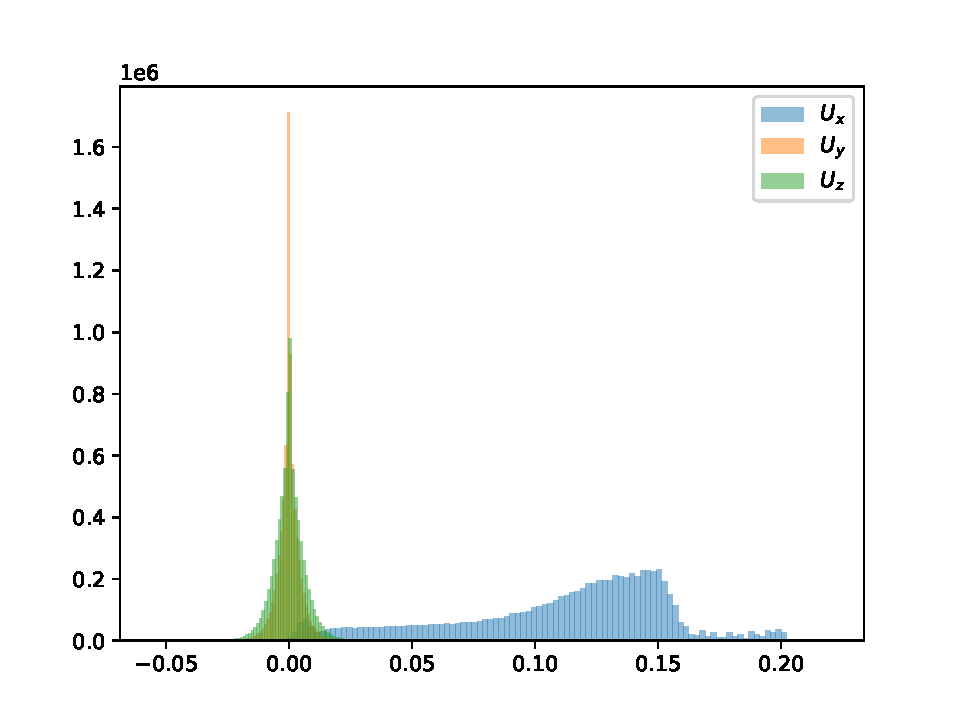
\includegraphics{fig/U_hist.pdf}
		\label{fig:U_hist}
		\caption{Histogram plot of the velocity magnitude $U$}
	\end{figure}
\end{frame}

\begin{frame}{Dataset preprocessing}

\end{frame}



\begin{frame}{A priori test}
	\begin{itemize}
		\item The first approach usually provides a much better apriori error ($0.7$) estimate than the second approach.
	\end{itemize}
\end{frame}

\begin{frame}{A posteriori test}

\end{frame}

\begin{frame}{Future work}
	\begin{itemize}
		\item 1. Deploy to practical problems: Subgrid-scale modeling in large eddy simulation of the
		urban environment.
		\item 2. 
	\end{itemize}
\end{frame}

\begin{frame}{Dataset difference}
	The a-priori test does not show a big difference between training with different datasets.
\end{frame}

\end{document}